\chapter{Probability Problem set Solutions}
\begin{enumerate}
	\item An unbiased dice is thrown three times successively. The probability that the numbers of dots on the uppermost surface add up to 16 is
	{\exyear{NET/JRF(DEC-2011)}}
	\begin{tasks}(4)
		\task[\textbf{A.}] $\frac{1}{16}$
		\task[\textbf{B.}] $\frac{1}{36}$
		\task[\textbf{C.}] $\frac{1}{108}$
		\task[\textbf{D.}] $\frac{1}{216}$
	\end{tasks}
	\begin{answer}
		\begin{align*}
		\intertext{ We can get sum of dice as 16 in total six ways i.e. three ways $(6,5,5)$ and three ways $(6,6,4)$}
		\text{Total number of ways for 3 dice having six faces }&=6 \times 6 \times 6\\
		&=\frac{6}{6 \times 6 \times 6}=\frac{1}{36}
		\end{align*}
		So the correct answer is \textbf{Option (B)}
	\end{answer}
	\item A ball is picked at random from one of two boxes that contain 2 black and 3 white and 3 black and 4 white balls respectively. What is the probability that it is white?
	{\exyear{NET/JRF(JUNE-2012)}}
	\begin{tasks}(4)
		\task[\textbf{A.}] $34 / 70$
		\task[\textbf{B.}] $41 / 70$
		\task[\textbf{C.}] $36 / 70$
		\task[\textbf{D.}] $29 / 70$
	\end{tasks}
	\begin{answer}$\left. \right. $
		\begin{figure}[H]
			\centering
			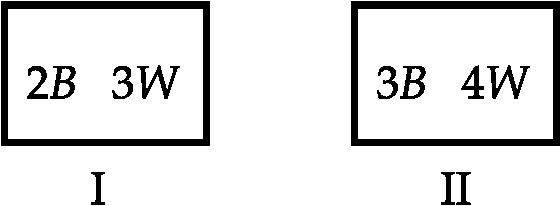
\includegraphics[height=1.6cm,width=4.55cm]{NET-19-2012}
		\end{figure}
		\begin{align*}
		\intertext{Probability of picking white ball}
		\text{From box }I=\frac{3}{5} \text{ and from box }I I&=\frac{4}{7}
		\intertext{Probability of picking a white ball from either of the two boxes is $=\frac{1}{2}\left[\frac{3}{5}+\frac{4}{7}\right]=\frac{41}{70}$}
		\end{align*}
		So the correct answer is \textbf{Option (B)}
	\end{answer}
	\item  A bag contains many balls, each with a number painted on it. There are exactly $n$ balls which have the number $n$ (namely one ball with 1 , two balls with 2, and so on until $N$ on them). An experiment consists of choosing a ball at random, noting the number on it and returning it to the bag. If the experiment is repeated a large number of times, the average value the number will tend to
	{\exyear{NET/JRF(JUNE-2012)}}
	\begin{tasks}(4)
		\task[\textbf{A.}] $\frac{2 N+1}{3}$
		\task[\textbf{B.}] $\frac{N}{2}$
		\task[\textbf{C.}] $\frac{N+1}{2}$
		\task[\textbf{D.}] $\frac{N(N+1)}{2}$
	\end{tasks}
	\begin{answer}
		\begin{align*}
		\text{Total number of balls }1+2+3+4+\ldots . .+N&=\frac{N(N+1)}{2}\\
		\text{The probability for choosing a $k^{\text {th }}$ ball at random } &=\frac{k}{\frac{N(N+1)}{2}}\\
		\text{Average of it is given by }\langle k\rangle&=\Sigma k \cdot P=\frac{2 \Sigma k^{2}}{N(N+1)}\\&=\frac{2}{N(N+1)} \cdot \frac{N(N+1)(2 N+1)}{6}\\
		&=\frac{2 N+1}{3} \quad\text{ where }\Sigma k^{2}=\frac{N(N+1)(2 N+1)}{6}
		\end{align*}
		So the correct answer is \textbf{Option (A)}
	\end{answer}
	\item  In a series of five Cricket matches, one of the captains calls "Heads" every time when the toss is taken. The probability that he will win 3 times and lose 2 times is
	{\exyear{NET/JRF(DEC-2012)}}
	\begin{tasks}(4)
		\task[\textbf{A.}] $1 / 8$
		\task[\textbf{B.}]  $5 / 8$
		\task[\textbf{C.}] $3 / 16$
		\task[\textbf{D.}] $5 / 16$
	\end{tasks}
	\begin{answer}
		\begin{align*}
		P&=\left(\frac{1}{2}\right)^{3}\left(1-\frac{1}{2}\right)^{5-3} \frac{5 !}{3 !(5-3) !}\\&=\frac{1}{8} \times\left(\frac{1}{2}\right)^{2} \cdot \frac{5 !}{3 !(5-3) !}\\
		&=\frac{1}{32} \cdot \frac{5 \times 4 \times 3 !}{3 ! \times 2 !}=\frac{20}{32 \times 2}\\&=\frac{5}{8 \times 2}=\frac{5}{16}
		\intertext{The probability of getting exactly $k$ successes in $n$ trials is given by probability mass function $=\frac{n !}{k !(n-k) !} p^{k} \cdot(1-p)^{n-k}, k=$ successes, $n=$ trials.}
		\end{align*}
		So the correct answer is \textbf{Option (D)}
	\end{answer}
	\item  Two independent random variables $m$ and $n$, which can take the integer values $0,1,2, \ldots, \infty$, follow the Poisson distribution, with distinct mean values $\mu$ and $v$ respectively. Then
	{\exyear{NET/JRF(DEC-2014)}}
	\begin{tasks}(1)
		\task[\textbf{A.}]  The probability distribution of the random variable $l=m+n$ is a binomial distribution.
		\task[\textbf{B.}] The probability distribution of the random variable $r=m-n$ is also a Poisson distribution.
		\task[\textbf{C.}] The variance of the random variable $l=m+n$ is equal to $\mu+v$
		\task[\textbf{D.}] The mean value of the random variable $r=m-n$ is equal to 0 
	\end{tasks}
	\begin{answer}
		\begin{align*}
		\sigma_{l}^{2}&=\sigma_{m}^{2}+\sigma_{n}^{2}=\mu+v
		\end{align*}
		So the correct answer is \textbf{Option (C)}
	\end{answer}
	\item  Consider a random walker on a square lattice. At each step the walker moves to a nearest neighbour site with equal probability for each of the four sites. The walker starts at the origin and takes 3 steps. The probability that during this walk no site is visited more than one is
	{\exyear{NET/JRF(DEC-2015)}}
	\begin{tasks}(4)
		\task[\textbf{A.}] $12 / 27$
		\task[\textbf{B.}] $27 / 64$
		\task[\textbf{C.}] $3 / 8$
		\task[\textbf{D.}] $9 / 16$
	\end{tasks}
	\begin{answer}
		\begin{align*}
		\text{Total number of ways }&=4 \times 4 \times 4\\
		\text{Number of preferred outcome }&=4 \times 3 \times 3
		\intertext{$(\because$ Any four option in step-1 and only 3 option in step $2 \& 3$ because he can not go to previous position)}\\
		\text{probability }&=\frac{4 \times 3 \times 3}{4 \times 4 \times 4}=\frac{9}{16}
		\end{align*}
		So the correct answer is \textbf{Option (D)}
	\end{answer}
	\item  Let $X$ and $Y$ be two independent random variables, each of which follow a normal distribution with the same standard deviation $\sigma$, but with means $+\mu$ and $-\mu$, respectively. Then the sum $X+Y$ follows a
	{\exyear{NET/JRF(JUNE-2016)}}
	\begin{tasks}(1)
		\task[\textbf{A.}] Distribution with two peaks at $\pm \mu$ and mean 0 and standard deviation $\sigma \sqrt{2}$
		\task[\textbf{B.}]  Normal distribution with mean 0 and standard deviation $2 \sigma$
		\task[\textbf{C.}] Distribution with two peaks at $\pm \mu$ and mean 0 and standard deviation $2 \sigma$
		\task[\textbf{D.}] Normal distribution with mean 0 and standard deviation $\sigma \sqrt{2}$
	\end{tasks}
	\begin{answer}
		\begin{align*}
		\mu^{\prime}&=\mu_{x}+\mu_{y}=\mu-\mu=0\\
		\sigma^{12}&=\sigma_{x}^{2}+\sigma_{y}^{2}=\sigma^{2}+\sigma^{2}\\
		\sigma^{\prime}&=\sqrt{2} \sigma
		\end{align*}
		So the correct answer is \textbf{Option (D)}
	\end{answer}
	\item  A random variable $n$ obeys Poisson statistics. The probability of finding $n=0$ is $10^{-6}$. The expectation value of $n$ is nearest to
	{\exyear{NET/JRF(JUNE-2017)}}
	\begin{tasks}(4)
		\task[\textbf{A.}] 14
		\task[\textbf{B.}] $10^{6}$
		\task[\textbf{C.}] $e$
		\task[\textbf{D.}] $10^{2}$
	\end{tasks}
	\begin{answer}
		\begin{align*}
		\intertext{In Poisson's statistics the probability of finding the value $n$ is given by $P(n)=\frac{\mu^{n}}{n !} e^{-\mu}$}
		\intertext{The mean of Poisson's statistics is $\mu$. From the question}
		P(0)&=10^{-6} \Rightarrow 10^{-6}=\frac{\mu^{0}}{0 !} e^{-\mu} \Rightarrow e^{-\mu}=10^{-6}\\
		\text{	Talking Log of both sides, }-\mu&=-6 \ln 10 \Rightarrow \mu=6 \ln 10\\
		\text{Hence the expectation value of $n$ is }\mu&=6 \times 2.30=13.8 \approx 14
		\end{align*}
		So the correct answer is \textbf{Option (A)}
	\end{answer}
\item At each time step, a random walker in one dimension either remains at the same point with probability $\frac{1}{4}$, or moves by a distance $\Delta$ to the right or left with probabilities $\frac{3}{8}$ each. After $N$ time steps, its root mean squared displacement is
{\exyear{NET/JRF(JUNE-2019)}}
\begin{tasks}(4)
	\task[\textbf{A.}] $\Delta \sqrt{N}$
	\task[\textbf{B.}] $\Delta \sqrt{\frac{9 N}{16}}$
	\task[\textbf{C.}] $\Delta \sqrt{\frac{3 N}{4}}$
	\task[\textbf{D.}] $\Delta \sqrt{\frac{3 N}{8}}$
\end{tasks}
\begin{answer}
	\begin{align*}
	\intertext{For this problem it is evident from problem and given options}
	x_{\mathrm{rms}}&=k \sqrt{N}\\
	\text{If }N&=1 \text{ (Special case) (Let)}
	\intertext{Outcomes $1,0,-1$
		(times $\Delta$ ) with probability $\frac{3}{8}, \frac{1}{4}, \frac{3}{8}$}
	\left\langle x^{2}\right\rangle&=\sum P_{i} X_{i}^{2}=\frac{3}{8} \cdot 1+\frac{1}{4} \cdot 0+\frac{3}{8} \cdot 1\\&=\frac{3}{4} \Rightarrow x_{\text {rms }}=\sqrt{\frac{3}{4} \cdot 1}\\
	\text{So, option }&\Delta \sqrt{\frac{3 N}{4}}\text{ is correct.}
	\end{align*}
	So the correct answer is \textbf{Option (C)}
\end{answer}
	\item A box contains 5 white and 4 black balls. Two balls are picked together at random from the box. What is the probability that these two balls are of different colours?
	{\exyear{NET/JRF(DEC-2019)}}
	\begin{tasks}(4)
		\task[\textbf{A.}] $\frac{1}{2}$ 
		\task[\textbf{B.}] $\frac{5}{18}$
		\task[\textbf{C.}] $\frac{1}{3}$
		\task[\textbf{D.}] $\frac{5}{9}$
	\end{tasks}
	\begin{answer}
		\begin{align*}
		\intertext{Probability that the two balls are of different colors}
		&5 W, 4 B\\
		&=\frac{5 C_{1} \times 4 C_{1}}{9 C_{2}}=\frac{\frac{5 !}{4 ! \times 1 !} \times \frac{4 !}{3 ! \times 1 !}}{\frac{9 !}{7 ! \times 2 !}}=\frac{5 \times 4}{\frac{9 \times 8}{2}}=\frac{5}{9}
		\end{align*}
		So the correct answer is \textbf{Option (D)}
	\end{answer}
	\item  A particle hops randomly from a site to its nearest neighbour in each step on a square lattice of unit lattice constant. The probability of hopping to the positive $x$-direction is $0.3$, to the negative $x$-direction is $0.2$, to the positive $y$-direction is $0.2$ and to the negative $y$-direction is $0.3 .$ If a particle starts from the origin, its mean position after $N$ steps is
	{\exyear{NET/JRF(DEC-2019)}}
	\begin{tasks}(4)
		\task[\textbf{A.}] $\frac{1}{10} N(-\hat{i}+\hat{j})$
		\task[\textbf{B.}] $\frac{1}{10} N(\hat{i}-\hat{j})$
		\task[\textbf{C.}] $N(0.3 \hat{i}-0.2 \hat{j})$
		\task[\textbf{D.}] $N(0.2 \hat{i}-0.3 \hat{j})$
	\end{tasks}
	\begin{answer}
		\begin{align*}
		&\left\langle r_{i}\right\rangle \sum_{i} p_{i} r_{i}\\
		&=0.3 \hat{i}-0.2 \hat{i}+0.2 j-0.3 \hat{j}=0.1 \hat{i}-0.1 \hat{j}\\
		\text{For $N$ steps, }&=\frac{N}{10}[\hat{i}-\hat{j}]
		\end{align*}
		So the correct answer is \textbf{Option (B)}
	\end{answer}
	\item A basket consists of an infinite number of red and black balls in the proportion $p:(1-p)$. Three balls are drawn at random without replacement. The probability of their being two red and one black is a maximum for
	{\exyear{NET/JRF(JUNE-2020)}}
	\begin{tasks}(4)
		\task[\textbf{A.}]  $p=\frac{3}{4}$
		\task[\textbf{B.}] $p=\frac{3}{5}$
		\task[\textbf{C.}] $p=\frac{1}{2}$
		\task[\textbf{D.}] $p=\frac{2}{3}$
	\end{tasks}
	\begin{answer}
		\begin{align*}
		P&=p^{2}(1-p) \quad \\&\Rightarrow \frac{d P}{d p}=\frac{d}{d p} p^{2}(1-p)=0 \\&\Rightarrow p^{2}(-1)+(1-p) 2 p=0\\
		&\Rightarrow-p^{2}+2 p-2 p^{2}\\&=0 \Rightarrow 3 p^{2}=2 p \Rightarrow p=2 / 3
		\end{align*}
		So the correct answer is \textbf{Option (D)}
	\end{answer}
	
	
	
	
	
	
	
	
	
	
	
	
	
	
	\item An unbiased die is cast twice. The probability that the positive difference (bigger smaller) between the two numbers is 2 is
	{\exyear{ JEST 2012}}
	 \begin{tasks}(2)
		\task[\textbf{a.}]$\frac{1}{9}$
		\task[\textbf{b.}]$\frac{2}{9}$
		\task[\textbf{c.}] $\frac{1}{6}$
		\task[\textbf{d.}] $\frac{1}{3}$
	\end{tasks}
	\begin{answer}
		\begin{align*}
		p(2)&=\frac{n(E)}{n(S)}
		\intertext{The number of ways to come positive difference}
		&[(3,1),(4,2),(5,3),(6,4),(1,3)(2,4),(3,5)(4,6)]\\
		p(2)&=\frac{8}{36}=\frac{2}{9}
		\end{align*}
		So the correct answer is \textbf{Option (b)}
	\end{answer}
	\item A box contains 100 coins out of which 99 are fair coins and 1 is a double-headed coin. Suppose you choose a coin at random and toss it 3 times. It turns out that the results of all 3 tosses are heads. What is the probability that the coin you have drawn is the doubleheaded one?
	{\exyear{ JEST 2013}}
	 \begin{tasks}(2)
		\task[\textbf{a.}] $0.99$
		\task[\textbf{b.}]$0.925$
		\task[\textbf{c.}] $0.75$
		\task[\textbf{d.}] $0.01$
	\end{tasks}
	\begin{answer}
		So the correct answer is \textbf{Option (c)}
	\end{answer}
	\item There are on average 20 buses per hour at a point, but at random times. The probability that there are no buses in five minutes is closest to
	{\exyear{ JEST 2013}}
	 \begin{tasks}(2)
		\task[\textbf{a.}]$0.07$
		\task[\textbf{b.}] $0.60$
		\task[\textbf{c.}]$0.36$
		\task[\textbf{d.}] $0.19$
	\end{tasks}
	\begin{answer}
		\begin{align*}
		\intertext{From Poision's distribution function,}
		P(n)&=\frac{e^{-\lambda} \lambda^{n}}{\lfloor n}
		\text{here, }\lambda&=20\text{ buses per hour }\\
		\Rightarrow \lambda&=\frac{5}{3}\text{ buses in five minutes}
		\intertext{Therefore, the probability that there are no buses in five minutes,}
		P(n=0)&=\frac{e^{-\frac{5}{3}}\left(\frac{5}{3}\right)^{0}}{\lfloor 0}=e^{-5 / 3}=0.1886 \approx 0.19
		\end{align*}
		So the correct answer is \textbf{Option (d)}
	\end{answer}
	\item Two drunks start out together at the origin, each having equal probability of making a step simultaneously to the left or right along the $x$ axis. The probability that they meet after $n$ steps is
	{\exyear{ JEST 2013}}
	 \begin{tasks}(2)
		\task[\textbf{a.}]$\frac{1}{4^{n}} \frac{2 n !}{n !^{2}}$
		\task[\textbf{b.}] $\frac{1}{2^{n}} \frac{2 n !}{n !^{2}}$
		\task[\textbf{c.}] $\frac{1}{2^{n}} 2 n !$
		\task[\textbf{d.}]  $\frac{1}{4^{n}} n !$
	\end{tasks}
	\begin{answer}
		\begin{align*}
		\text{The probability of taking ' $r$ '}&\text{ steps out of $N$ steps }={ }^{N} C_{r}\left(\frac{1}{2}\right)^{r}\left(\frac{1}{2}\right)^{N-r}\\
		\text{Total steps }&=N=n+n=2 n
	\intertext{	For taking probability of $n$ steps out of $N$}
	P={ }^{N} C_{n}\left(\frac{1}{2}\right)^{n}\left(\frac{1}{2}\right)^{N-n}&=\frac{N !}{(N-n) ! n !}\left(\frac{1}{2}\right)^{n}\left(\frac{1}{2}\right)^{N-n}=\frac{2 n !}{n ! n !}\left(\frac{1}{2}\right)^{2 n}=\frac{2 n !}{(n !)^{2} 4^{n}}
		\end{align*}
		So the correct answer is \textbf{Option (a)}
	\end{answer}
	\item If two ideal dice are rolled once, what is the probability of getting atleast one '6'?
	{\exyear{ JEST 2015}}
	 \begin{tasks}(2)
		\task[\textbf{a.}]$\frac{11}{36}$
		\task[\textbf{b.}]$\frac{1}{36}$
		\task[\textbf{c.}]$\frac{10}{36}$
		\task[\textbf{d.}]  $\frac{5}{36}$
	\end{tasks}
	\begin{answer}
		\begin{align*}
		\text{Number of point}&\text{ in sample space } n(S)=11\\
		[(1,6),(2,6),(3,6),&(4,6),(5,6),(6,1),(6,2),(6,3),(6,4),(6,5),(6,6)]\\
	\text{	Number of point }&\text{in population }n(P)=6^{2}=36
		\intertext{Probability of getting atleast one '6' on face of dice} &=\frac{n(S)}{n(P)}=\frac{11}{36}
		\end{align*}
			So the correct answer is \textbf{Option (a)}
	\end{answer}
	\item The mean value of random variable $x$ with probability density $p(x)=\frac{1}{\sigma \sqrt{2 \pi}} . \exp \left[-\frac{\left(x^{2}+\mu x\right)}{\left(2 \sigma^{2}\right)}\right]$ is:
	{\exyear{ JEST 2016}}
	 \begin{tasks}(2)
		\task[\textbf{a.}]0
		\task[\textbf{b.}]$\frac{\mu}{2}$
		\task[\textbf{c.}] $\frac{-\mu}{2}$
		\task[\textbf{d.}]  $\sigma$
	\end{tasks}
	\begin{answer}
		\begin{align*}
		\langle x\rangle=\frac{1}{\sigma \sqrt{2 \pi}} \int_{-\infty}^{\infty} x \exp \left(-\frac{x^{2}}{2 \sigma^{2}}\right) d x \int_{-\infty}^{\infty} \exp \left(-\frac{\mu x}{2 \sigma^{2}}\right) d x=0 \quad\text{ (due to odd function)}
		\end{align*}
		So the correct answer is \textbf{Option (a)}
	\end{answer}
\item Suppose that we toss two fair coins hundred times each. The probability that the same number of heads occur for both coins at the end of the experiment is
{\exyear{ JEST 2017}}
 \begin{tasks}(2)
	\task[\textbf{a.}]$\left(\frac{1}{4}\right)^{100} \sum_{n=0}^{100}\left(\begin{array}{c}100 \\ n\end{array}\right)$
	\task[\textbf{b.}] $2\left(\frac{1}{4}\right)^{100} \sum_{n=0}^{100}\left(\begin{array}{c}100 \\ n\end{array}\right)^{2}$
	\task[\textbf{c.}]$\frac{1}{2}\left(\frac{1}{4}\right)^{100} \sum_{n=0}^{100}\left(\begin{array}{c}100 \\ n\end{array}\right)^{2}$
	\task[\textbf{d.}] $\left(\frac{1}{4}\right)^{100} \sum_{n=0}^{100}\left(\begin{array}{c}100 \\ n\end{array}\right)^{2}$
\end{tasks}
\begin{answer}
	\begin{align*}
	\intertext{ If we toss one fair coins hundred times, then probability of $n$ number of head occurs at the end of 100 times is}
	&{ }^{100} C_{n}\left(\frac{1}{2}\right)^{n}\left(\frac{1}{2}\right)^{100-n}
\intertext{	Hence, the probability that same number of heads occur for both coins at the end of experiment is}
&\sum_{n=0}^{100}\left({ }^{100} C_{n}\left(\frac{1}{2}\right)^{100}\right) \cdot\left({ }^{100} C_{n}\left(\frac{1}{2}\right)^{100}\right)=\sum_{n=1}^{100}\left({ }^{100} C_{n}\right)^{2}\left(\frac{1}{2}\right)^{200}=\left(\frac{1}{4}\right)^{100} \sum_{n=1}^{100}\left({ }^{100} C_{n}\right)^{2}
	\end{align*}
		So the correct answer is \textbf{Option (d)}
\end{answer}
\item An electronic circuit with 10000 components performs its intended function success fully with a probability $0.99$ if there are no faulty components in the circuit. The probability that there are faulty components is $0.05$. if there are faulty components, the circuit perform successfully with a probability $0.3$. The probability that the circuit performs successfully is $\frac{x}{10000}$. What is $x$ ?
{\exyear{ JEST 2018}}
\begin{answer}
So the correct answer is  \textbf{9555}
\end{answer}
\item A person plans to go from town $A$ to town $B$ by taking either the route $(R 1+R 2)$ with probability $\frac{1}{2}$ or the route $(R 1+R 3)$ with probability $\frac{1}{2}$ (see figure). Further, there is a probability $\frac{1}{3}$ that $R 1$ is blocked, a probability $\frac{1}{3}$ that $R 2$ is blocked, and a probability $\frac{1}{3}$ that $R 3$ is blocked. What is the probability that he/she would reach town $B$ ?
{\exyear{ JEST 2019}}
\begin{figure}[H]
	\centering
	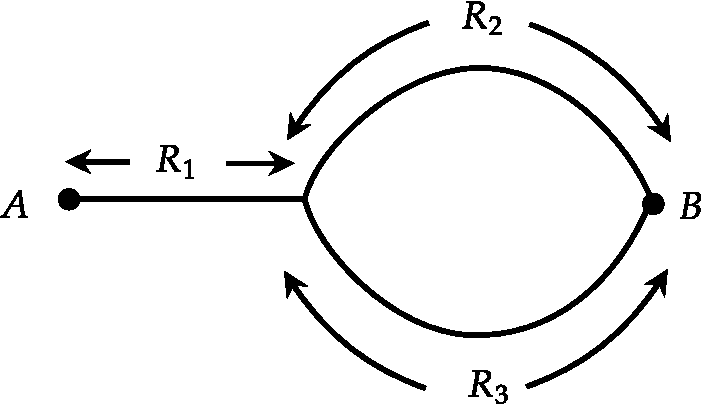
\includegraphics[height=3cm,width=5.5cm]{JEST-58-2019}
\end{figure}
 \begin{tasks}(2)
	\task[\textbf{a.}]$\frac{8}{9}$
	\task[\textbf{b.}]$\frac{1}{3}$
	\task[\textbf{c.}]$\frac{4}{9}$
	\task[\textbf{d.}]$\frac{2}{3}$
\end{tasks}
\begin{answer}
	\begin{align*}
	\text{Given that probability of}&\text{ $R 1$ blocked }=1 / 3\\
	\text{Probability of $R 1$ }&\text{not blocked }=1-\frac{1}{3}=\frac{2}{3}\\
	\text{Probability from $A$ to $B$ }&\text{without restriction }=\frac{1}{2}\\
	\text{Route $R 2$ probability }&=\frac{1}{2} \times \frac{2}{3}\text{ not blocked}\\
	\text{Route }R 3&=\frac{1}{2} \times \frac{2}{3}\\
\text{	Total probability }(A \rightarrow B)&=\frac{2}{3}\left[\frac{1}{2} \times \frac{2}{3}+\frac{1}{2} \times \frac{2}{3}\right]=\frac{4}{9}
	\end{align*}
	So the correct answer is \textbf{Option (c)}
\end{answer}

\end{enumerate}